\documentclass[11pt]{article}

\title{Building 3D Dense Reconstructions using LiDAR from a Walking Robot}
\author{Marcelo Gennari do Nascimento \\ Wadham College, University of Oxford}
\date{\today}

\usepackage{geometry}
 \geometry{
 a4paper,
 left=20mm,
 right=20mm,
 bottom=20mm,
 top=20mm,
 }
 
\setlength{\headheight}{14pt} 
\usepackage{setspace}
\usepackage{graphicx}
\usepackage[labelfont=bf]{caption}
\usepackage{amsmath}
\graphicspath{ {images/}}
\doublespacing

\begin{document}
	\pagenumbering{gobble}

	\maketitle

	\newpage
	\section*{Acknowledgments}
	\thispagestyle{empty}

	I like to aknowledge ...

	\clearpage
	\newpage

	\begin{abstract}
		Abstract text goes here
	\end{abstract}

	\newpage
	\tableofcontents

	\newpage
	\pagenumbering{arabic}
	\section{Introduction}
	\paragraph{}
	Autonomous robots are going to be one of the major achievements of science to the benefit of the public. Autonomy though depends on two main problems that are tightly related to each other: Localization and Mapping. The first concerns the problem of mapping the environment given a prior robot's trajectory. Most of the time though, neither the trajectory nor the map is known a priori.
	
	\paragraph{}
	Since the 1986 IEEE Robotics and Automation Conference, researchers have framed the general problem of Simultaneous Localization and Mapping (SLAM) as the ``holy grail" of modern robotics \cite{SLAMPartI}. A reliable solution to this problem would make autonomy one step closer to reality. Since the conference, a number of algorithms have been developed that successfully tackle SLAM, each of them with their advantages and drawbacks.

	\paragraph{}
	This project is concerned with putting together state of the art algorithms for SLAM and reconstruction systems to reliably and effiiciently build a 3D map of an environment with LiDAR data from a walking robot without any prior map or prior trajectory available. The success of this project would contribute to making the usage of mobile robots for tasks such as search and rescue and exploration one step closer to reality.

	\subsection{Aim of the Project}
	\subsection{ Organisation of the Report}
		\paragraph{Section 2} of the report will go through the literature review of the main building blocks of the project. In particular, we will explore the current developments in the solutions of the Simultaneous Localization and Mapping (SLAM), the Iterative Closest Points (ICP) and 3D Reconstruction problem.
		
		\paragraph{Section 3} will go deeper on the system pipeline of the project. In order to get a general understanding of the system, detaied explanation of the steps of data processing, inputting and outputting will be explained. This will also introduce the two main parts of the system that will be explained in subsequent sections.
		
		\paragraph{Section 4} explores the solution of the SLAM problem adopted in the project. Since building an accurate map is an essential step to the success of the project, this section will explain the details of how the SLAM solution works and why this particular structure was chosen.
		
		\paragraph{Section 5} shows how the output from the SLAM solution will be integrated with the 3D reconstruction system.
		
		\paragraph{Section 6} will conclude the report with an overall evaluation of how the system performed. It will also indicate ways in which the system could be improved in a subsequent project. An analysis of how the outcome of this project compares with similar systems will be provided.

	\newpage
	\section{Literature Review}
	\subsection{Simultaneous Localization and Mapping (SLAM)}
	\paragraph{}
	SLAM is the problem of whether it is possible for a mobile robot to create a globally consistent map of an environment and localize itself on it without prior knowledge of the map \cite{SLAMPartI}\cite{Cadena}. Building a map of an environment is a crucial step towards autonomy, since planning and control assume prior knowledge of mapping and localization. Mathematically, we can frame SLAM as a Markov Chain, a Bayes Net or a Factor Graph. Defining:
	
	\begin{itemize}
		\item $\mathbf{x_k}$: the pose of the robot (being $\mathbf{X_{0:k}}$ as the poses from time $\mathbf{0}$ to $\mathbf{k}$)
		\item $\mathbf{u_k}$: the odometry measurement ($\mathbf{U_{0:k}}$ as the historical measurements)
		\item $\mathbf{l_k}$: the landmark observation ($\mathbf{L_{0:k}}$ as the historical landmarks)
		\item $\mathbf{c_k}$: the loop closures
	\end{itemize}

	It is possible to formulate the problem of SLAM more formally using both a factor graph or a probabilistic framework:

	\begin{figure}[h]
		\centering
		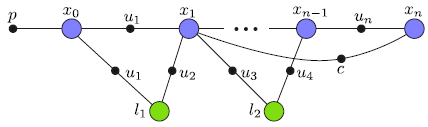
\includegraphics{SLAMFactorGraph.png}
		\caption{SLAM as a Factor Graph. The value $\mathbf{p}$ denotes a prior; $\mathbf{x_n}$ denotes the state vector; $\mathbf{u_n}$ denotes odometry measurements; $\mathbf{c}$ denotes close loops; $\mathbf{l_n}$ denotes landmark positions.}
		\label{fig:slam1}
	\end{figure}
	
	\paragraph{}
	The graph shown in Figure \ref{fig:slam1} is a Factor Graph representation of the dependencies between variables and measurements. A probabilistic framework can then be extracted from it. 
	\begin{equation}
	P(X,L,U,Z,C)\ \propto \ P(x_0)\prod_{i=1}^{M}P(x_i|x_{i-1}, u_i)\prod_{k=1}^{K}P(z_k|x_{i_k},l_{j_k})\prod_{w=1}^{W}P(x_i|x_{i_w}, c_w)
	\label{probSLAMeq}
	\end{equation}
	\paragraph{}
	The general goal of probabilistic SLAM is to find variables $\mathbf{X^*}$ and $\mathbf{L^*}$ that maximizes the posterior probability distribution of the Equation \ref{probSLAMeq}. Also, for the rest of this chapter, it will be assumed that the data association problem is solved and the indices $i_w$ and $i_k$ are known. 

	\paragraph{}
	Theoretically, the mathematical analysis of SLAM has been shown that it is indeed feasible to build a nondivergent map with no prior information, so it is widely accepted that in theoretical grounds, SLAM is a solved problem \cite{SLAMPartI}\cite{Cadena}\cite{CsorbaThesis}\cite{938381}. However, there are computational and algorithmic challenges that hinders the development of a real-time implementation system that performs SLAM. This problem gets even more complicated when considering unstructured environments and large scale maps \cite{SLAMPartII}.
	
	\paragraph{}
	There are three main implementations of SLAM: Kalman Filtering and Extended Kalman Filtering (with early works such as proposed by R. Smith \cite{Smith:1990:EUS:93002.93291}), Rao-Blackwellized Particle Filtering (most notably with FastSLAM \cite{Montemerlo02fastslam:a}) and Information Filter (with the now state-of-the-art work of iSAM from Michael Kaess \cite{Kaess08tro}).

	\subsubsection{Kalman Filtering}
	\paragraph{}
	As one of the first implementations to appear to solve the problem of SLAM, the Extended Kalman Filtering (EKF) approach makes two assumptions when formulating the probabilistic SLAM: the process model (also referred to motion model in mobile robotics) and the observation model.
	
	\begin{minipage}{.5\linewidth}
		\centering
		\begin{equation*}
		\begin{split}
		\mathbf{Process\ Model:} \\ 
		x_i = f(x_{i-1}, u_i) + w_i
		\end{split}
		\end{equation*}
	\end{minipage}
	\begin{minipage}{.5\linewidth}
		\centering
		\begin{equation*}
		\begin{split}
		\mathbf{Observation\ Model:} \\ 
		z_i = h(x_{i_k}, l_{j_k})+ + v_k
		\end{split}
		\end{equation*}
	\end{minipage}

	\paragraph{}
	where $w_i$ is white noise with covariance $Q$ and $v_k$ is white noise with covariance $R$. The process (motion) model is usually a generalization of how the robot moves (kinematics) \cite{Montemerlo02fastslam:a}\cite{772544}. As a consequence, the probability distributions $p(x_i|x_{i-1}, u_i)$ and $p(z_i|x_i, l_i)$ can be modeled as Gaussians with mean $f$ and $h$ and covariances $Q$ and $R$. Modern analysis of the SLAM algorithms have shown that due to linearization of the functions $f$ and $h$, assumptions about Gaussian noises and time-dependence of the process and observation model can cause the EKF solution to perform poorly unless many loop closures are detected in frequent intervals \cite{doi:10.1177/1729881416669482}.


	\paragraph{}
	It is also known that the Kalman Filter approach requires storage of the order of $O(N^2)$ (where $N$ is the number of features), and for a classic implementation of the algorithm, it also requires computational power of the order of $O(N^2)$ \cite{CsorbaThesis}. New methods for computing the covariances (which cause the squared dependence) by exploring state augmentation, partitioned updates and sparsity in the matrices have demonstrated faster solutions, thus requiring less computational power \cite{SLAMPartII}.

	\subsubsection{Particle Filtering}
	\paragraph{} \cite{Montemerlo02fastslam:a}\cite{772544}
	
	\subsubsection{Information Filter}
	\subsection{Iterative Closest Points (ICP)}
	\subsection{3D Reconstruction Systems}

	\newpage
	\section{System Pipeline} \label{pipeline}
	\paragraph{}
	The pipeline for the overall system can be seen below. It consists of 4 modules: (I) First odometry estimates (based on either Visual Odometry or Wheel Odometry); (II) Laser Odometry (using Simona Nobili's AICP \cite{7989547}); (III) Loop closure detection and Graph Optimization (using iSAM \cite{Kaess08tro}); (IV) 3D dense volumetric reconstruction (using BOR\textsuperscript{2}G-CUBES \cite{TannerFSR2015}\cite{TannerArXiv2016}).

	\paragraph{}
	These 4 modules are broken down in two parts: the first part is concerned about solving the SLAM problem, which outputs a reliable trajectory and map. The second part is concerned about inputting that to a 3D reconstruction system (which in this case if BOR\textsuperscript{2}G-CUBES) to build the environment volumetrically.

	\newpage
	\section{SLAM Solution}
	\paragraph{}
	As already introduced in Section \ref{pipeline}, the SLAM solution has 4 independent building blocks. This offers flexibility enough to test the effect that each part has in the outcome of the map. This section is going to discuss deeper how the solution works with all the building blocks working together. 
	 
	\subsection{First Odometry Measurements}
	\paragraph{}
	The first odometry measurements offer a relatively innacurate estimation of the pose of the robot at a certain time. It is used as the input pose to the AICP algorithm in order for it to process laser odometry based on the LiDAR scan.
	
	\paragraph{}
	During the project, two mehods to get the first odometry measurements were used. When getting data with the mobile robot Husky \cite{Husky}, the wheel odometry provided by the system served as a good first estimate of its position. When getting the data with the MultiSense SL \cite{multisense}, Visual Odometry from MultiSense's stereo camera was performed to get the first odometry estimations. 
	A graph of both paths in world coordinates are shown below for comparison, along with the LiDAR scans viewed at bird-view:
	
	\subsection{Laser Odometry}
	\paragraph{}
	Given the first odometry measurements, the AICP algorithm was used to incorporate the LiDAR scan of each of the paths to the estimation problem. For the Husky example, the Velodyne \cite{velodyne} LiDAR was used, whereas for the Oxford Dataset, the MultiSense SL LiDAR was used.
	
	\paragraph{}
	The results for each of the paths are shown below for comparison. It is noticeable the difference between the accuracy of the First Odometry Measurements to the Laser Odometry. However, it can be seen that there is drift due to how the AICP algorithm works.
	
	\subsection{Loop Closure Detection}
	\paragraph{}
	In order to adjust for the innacuracies of the path estimate, a loop closure detection algorithm was placed. Since it was assumed that the robot would not overdrift, three simple heuristics were used to detect loop closure: Time Filter Sampling, Euclidean Distance, and Pose Alignment. 
	\begin{itemize}
		\item \textbf{Filter Sampling:} In order to avoid the problem of loop closing two state estimates that are in the same room but did not leave the room, a time filter sampling was applied. The idea is to sample every $S$ state estimates, so that the candidate loop closing states would be sparse enough so that the loop just occurs between big time frames, but dense enough to apply euclidean distance.
		\item \textbf{Euclidean Distance:} Once the estimates have been  sampled, the euclidean distance between each of them is applied. If the distance between any two states is less than a threshold value $E$, then the two estimates form a candidate pair and they are added in the candidate pair list.
		\item \textbf{Pose Alignment:} After the resampling, the candidates pairs are tested for their relative pose. Since the loop closure correction relies on alignment of point clouds using ICP, it is a good strategy to select poses that would maximize the overlap between the point clouds associated with the candidates. In order to do that, another resampling is done based on the overlap between the field of view of the estimates. If the overlap is less than a threshold value $O$, then the candidate pair is dropped out from the list, and the remaining are the loop closures that are considered.
	\end{itemize}
	
	\paragraph{}
	The parameters $S$, $E$ and $O$ are chosen by hand depending on what dataset is used in the algorithm. Changing the parameters can affect the outcome of the map significantly, so it is important to spend some time tuning them to the specific requirements of the test.

	\subsection{Graph Optimization}

	\newpage
	\section{Integration with BOR\textsuperscript{2}G-CUBES}
	
	\newpage
	\section{Conclusion}

	\newpage
	\bibliography{4YPReportBibl}
	\bibliographystyle{ieeetr}

\end{document}
